\documentclass{letask}

\begin{document}
\begin{titlepage}
\center % Center everything on the page
 
%----------------------------------------------------------------------------------------
%	HEADING SECTIONS
%----------------------------------------------------------------------------------------

\textsc{\LARGE Московский\\[-0.2cm]Физико-Технический Институт\\[0.1cm]\large (государственный университет)}\\[1.5cm] % Name of your university/college
\textsc{\Large Кафедра общей физики}\\[0.1cm] % Major heading such as course name
\textsc{\large Лабораторная работа \textnumero  4.4.1}\\[0.5cm] % Minor heading such as course title

%----------------------------------------------------------------------------------------
%	TITLE SECTION
%----------------------------------------------------------------------------------------

\HRule
\\[0.4cm]
{ \huge \bfseries Амплитудная\\[0.2cm]
дифракционная решетка}
\\[0.6cm] % Title of your document
\HRule
\\[1.5cm]


 
%----------------------------------------------------------------------------------------
%	AUTHOR SECTION
%----------------------------------------------------------------------------------------

\begin{minipage}{0.4\textwidth}
	\begin{flushleft} \large
		\textsf{Студент}
		
		Ришат \textsc{Исхаков} \\[-0.15cm]
		513 группа
	\end{flushleft}
\end{minipage}
~
\begin{minipage}{0.4\textwidth}
	\begin{flushright} \large
		\textsf{Преподаватель}
		
		Александр Александрович \\[-0.15cm]
		\textsc{Казимиров} % Supervisor's Name
	\end{flushright}
\end{minipage}

\begin{bottompar}
	\begin{center}
		
\includegraphics[width = 80 mm]{logo.jpg}
	\end{center}
	{\large \today}

\end{bottompar}
\vfill % Fill the rest of the page with whitespace

\end{titlepage}

\textbf{Цель работы:}
изучение интерферометра Фабри-Перо и определение его характеристик, как спектрального прибора.
\textbf{В работе используются:} интерферометры Фабри-Перо, линзы, светофильтр, ртутная лампа ПРК-2, высокочастотная натриевая лампа, катетометры КМ-6.



\section{Теоретическая часть}

\subsection*{Интерферометр Фабри-Перо}

\begin{wrapfigure}[10]{r}{8 cm}
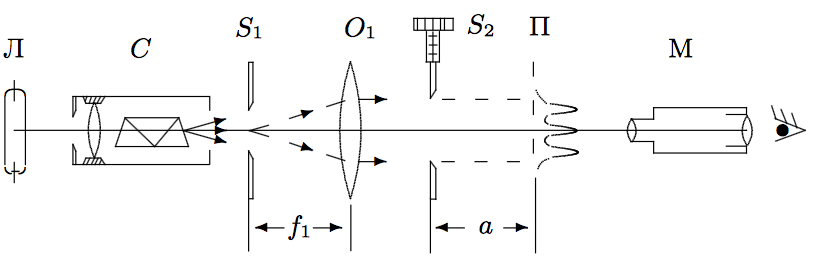
\includegraphics[width = 8 cm]{img1}
\caption{Интерферометр Фабри-Перо}
\end{wrapfigure}

Интерферометр Фабри-Перо состоит из двух отражающих пластин, внутренние поверхности которых хорошо отполированы и установлены параллельно друг другу. Его можно рассматривать как плоскопараллельную воздушную пластину, на которой происходят многократные отражения и интерференция световых лучей. Интерференционная картина, наблюдаемая в фокальной плоскости линзы Л, состоит из концентрических колец. 
Для двух соседних лучей, распространяющихся между зеркалами интерферометра под углом $\theta$, разность хода определяется соотношением
 
\begin{equation}
\Delta = 2 L \cos \theta,
\label{eq:dif}
\end{equation}

где $L$~--~расстояние между зеркалами интерферометра.
Будем считать, что поглощение света в зеркалах отсутствует, что достигается лишь при целых значениях отношения $\Delta / \lambda$.

Интерференционная картина состоит из узких светлых колец, разделенных широкими промежутками, расстояния между которыми мы будем измерять.

\subsection*{Измерение длин волн $\lambda$ и расстояний $d \lambda$ между спектральными линиями.}

Исследуем диаметры интерференционных колец, предполагая, что угол $\theta$ достаточно мал.
Рассмотрим два кольца с разным порядком интерференции: $m_i$ и $m_j$ соответственно. 
Из~(\ref{eq:dif}) и условия отсутствия поглощения следует, что светлое кольцо порядка $m$ образуется при 

\begin{equation}
\Delta = 2 L \cos \theta = m \lambda \; (m - \text{целое}).
\end{equation}


\section{Установка и параметры измерения}



\section{Вывод}


\end{document}
